\section{Design}
\label{sec:design}

Waskern is a file-oriented storage kernel that lets users define how reads and
writes affect their files.  As far as applications are concerned, Waskern looks
and behaves like a set of globally-available volumes, each of which contains a
mountable filesystem. Each user owns one or more volumes, and owns zero or more
files within volumes they can access.  A volume's file and structure is replicated across
multiple services, and its metadata and directory hierarchy is cached in a
scalable but untrusted PaaS provider.

In Waskern, a volume is a unit trust domain, and a user is a unit
administrative domain that encompasses one or more devices.  A volume has an
owner who has volume-level control over who may read and write files, and who
may process I/O flows. Volume users trust the volume owner to make appropriate
volume-wide decisions, but retain fine-grained control over who may read, write,
and process I/O for their files, as well as what I/O logic runs on their
devices.

\begin{figure}[t!]
\centering
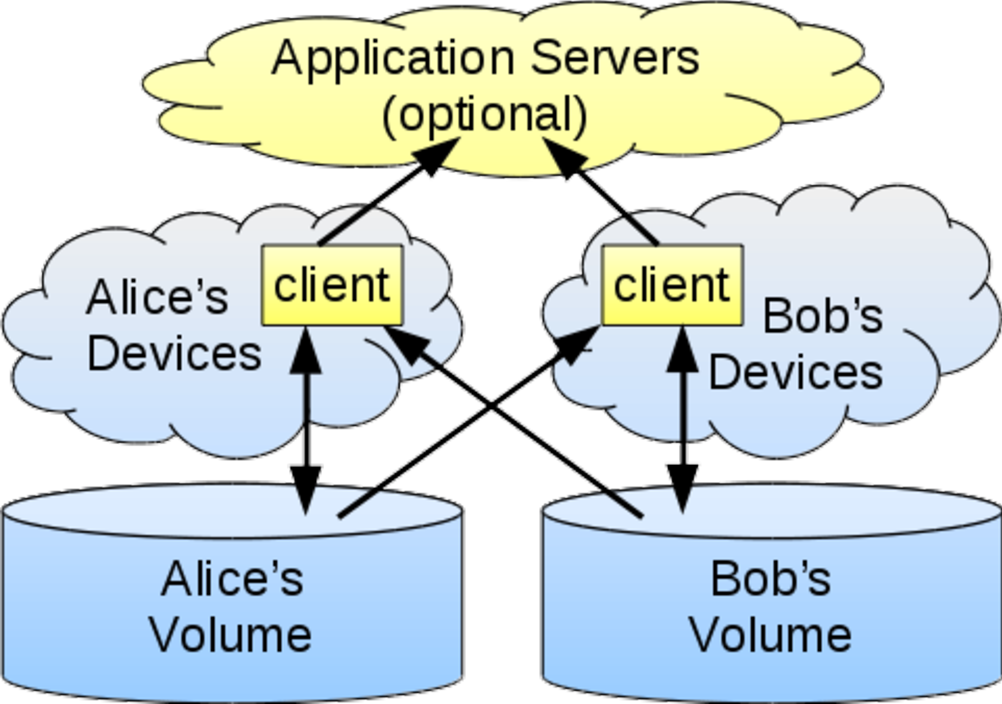
\includegraphics[width=0.47\textwidth]{figures/app-overview}
\caption{\it
Waskern gives each user an ``always-on'' data store that programmatically
hosts and manages data according to user-specified logic.  Applications no
longer need to host data:  their clients access a user's data directly from storage,
and their servers obtain read-permission from the user and
index publicly-available data to enable data discovery.  Servers are optional if
   discovery is not a concern.}
\label{fig:app-overview}
\end{figure}

This organization offers a simple, powerful, and cost-effective way to build multi-user
applications. For example, consider a Waskern-powered social media alternative
to Facebook. To use the application, Alice and Bob each create a volume for
hosting their social data, and they give the application read-only access. Users
make things like photos and posts available by writing them to their volumes,
and the application's servers read the volumes in order to index their
contents and facilitate user and content discovery.

Users have direct control over the I/O handling in their volumes, so their data
will be stored and accessed exactly how the they want. For example, Alice is
privacy-conscious, so she has her volume automatically encrypt her data before
it leaves her computers, and delete data that has not been accessed in over a
year. Bob, however, wants to keep his data highly available, so he has his
volume split his data into erasure codes and replicate them to many cloud
storage providers. Bob used to use Facebook, so he additionally maps his old
Facebook data as a read-only tree in his volume to make it available to Alice.
All the while, Alice and Bob's I/O coordination algorithms stand apart from
each other, the application, and the storage services, ensuring that each
user's desired features are always present and activated.

The only roles the application fulfills are to help Alice and Bob discover one
another, and to offer a convenient but \textit{non-exclusive} way to view and modify the
data. When Alice and Bob become friends, they give each other read access to
some of each others' files. When Alice leaves the application, she denies
the application and all of her friends read access. The application never
interacts with the underlying services.

\subsection{Files}

Waskern processes an I/O flow (a read or a write) in terms of immutable
chunks. A chunk has a globally unique identifier, and is either a block or a
manifest. A block is a fixed-size opaque blob of data, and a manifest represents
a snapshot of the file's data in between two consecutive writes (e.g. like
an inode structure). Each file has a latest manifest that identifies its current
state.

This representation enables users to reason about a file's consistency and
durability independently of the underlying services. To do so, Waskern defines
data plane programmability in terms of five discrete stages, which are invoked
in reaction to application-initiated reads and writes:

\textbf{Prepare}: Determines the new manifest and new set of blocks for a file.

\textbf{Push}: Makes the new manifest and blocks durable by replicating them to underlying services.

\textbf{Publish}: Propagates knowledge of a manifest to all application endpoints.

\textbf{Discover}: Acknowledges a manifest's publication.

\textbf{Pull}: Fetches the new manifest's data and blocks.

A user can implement any consistency model by controlling the details of
\texttt{publish} and \texttt{discover}, and can implement any durability model
by controlling \texttt{push} and \texttt{pull}. For example, sequential
consistency can be achieved on a file by synchronously publishing and
discovering its manifest on each write and read, respectively. As another
example, causal consistency can be achieved by publishing and discovering the
file once, and then propagating vector clocks between readers and writers as
part of pushes and pulls. Because chunks are immutable and uniquely named, they
can be cached anywhere to improve performance without affecting correctness.

\subsection{Gateways}

Waskern grants users control over a set of execution contexts called
\textit{gateways}. Gateways are stand-alone,
asynchronous processors that run application-given data-plane processing logic
on reads and writes (achieving universality). Gateways can scale down to a
single process and scale up to multiple data centers (achieving uniformity).

Each user owns one or more gateways in a volume. Data enters Waskern from
users via an application or via an existing data source of the user's choice
(e.g. websites, cloud storage). Data gets stored into existing storage
providers, and is ultimately served back to users via a gateway or an
application that access it on their behalf. As such, Waskern defines three
types of gateway:

\textbf{Acquisition Gateway (AG)}: AGs map a 3rd party dataset into a volume as a read-only
file hierarchy.  They the view of the data synchronized with changes in the
external data source, and implement only the \texttt{publish} and \texttt{pull}
stages.

\textbf{Replica Gateway (RG)}:   RGs upload chunks from other gateways into existing
storage services, and serve them back out on request. They implement only the
``push'' and ``pull'' stages.

\textbf{User Gateway (UG)}: UGs interact with the
application and user, and initiate new flows on their behalf. They offer a control-plane interface directly to
users, in order for them to change the I/O logic and configuration at runtime.

UGs implement all five I/O stages. They generate new manifests and blocks on a
write-request from the application, push the new chunks and garbage-collect
overwritten chunks from RGs, and publish the new manifest to the volume. On read
requests, they discover manifests from UGs and AGs, and pull chunks from AGs and
RGs. They may communicate with other existing systems in order to do so (like
CDNs).

\begin{figure*}
\centering
\includegraphics[width=0.9\textwidth]{figures/volume-gateway}
\caption{\it Volumes are comprised of multiple gateways.  Bob shares both his
volume data and legacy Facebook data with Alice by granting her a read-only RG
to access his cloud storage providers, and a read-only UG to access his RG and
AG.  These gateways run Bob's I/O logic to do so, which Alice trusts.}
\label{fig:volume-gateway}
\end{figure*}

Using our social media example, Alice, Bob, and the application servers run UGs
to access data. The UGs implement the stable interfaces the application
expects--a userspace filesystem for its clients and a RESTful web API for its
servers. For privacy, Alice's UGs run logic to encrypt her chunks before
pushing them to RGs.

Alice and Bob do not need to run publicly-routable RGs. Instead, Bob creates
a read-only UG and RG for Alice, which she runs on her devices. Alice does
likewise for Bob.  Alice's other RGs will delete data on her cloud storage
providers, and Bob's other RGs create erasure codes from chunks and
replicate them widely.

Bob wants to make his previously-created data from Facebook available to Alice
and the application.  To do so, he deploys a publicly-routable AG in an IaaS
provider to map the data as a read-only directory tree. This way, Alice can
read it without interacting with Facebook, and Bob does not need to export his
Facebook data to make it available.
%I'm a little worried that also using the Facebook example here might
%give the wrong impression that everything is pairwise (between all pairs
%of Bob and Alice.

\subsection{Coordination}

Gateways coordinate I/O flows via a stateful control-plane, through which
Waskern achieves its programmability, dynamicity, and extensibility
properties. The control-plane state for each gateway includes its I/O logic,
owner, public key, host, port, and volume-given capabilities, as well as the
list of users and gateways that make up a volume. Waskern allows these fields
to be set at runtime, and ensures that a user's or volume owner's state
changes are atomic with respect to the I/O flows.

To implement its control plane, Waskern assigns each file a coordinator
gateway. The coordinator gateway decides when an I/O flow for that file starts
and finishes, and maintains the file's authoritative manifest. The specifics
of how the manifest is externalized are handled by the user-supplied publish I/O
stage, but coordinators always ensure that no I/O flow-processing occurs while
the control-plane state is being updated. Coordinator responsibility may be
passed between gateways to mask faults, optimize load distribution, and control
who manages a file's state and how they do it.


\begin{figure}[t!]
\centering
\includegraphics[width=0.47\textwidth]{figures/cert-graph}
\caption{\it
Overview of the cryptographic links within a certificate graph.
   }
\label{fig:cert-graph}
\end{figure}


The control plane concerns itself with managing causally-consistent
state-changes on a cryptographic store called a \textit{certificate graph}
(Figure~\ref{fig:cert-graph}). Each gateway
maintains a replica of the certificate graph, which it uses to verify the
relationships between users, gateway state, and file state in a non-repudiable
manner. The cryptographic hash of each file's blocks are incorporated into
their manifests, and each manifest is signed by the coordinator gateway that
prepared it. The state of each gateway is cryptographically signed by its user,
and the set of users and gateways in the volume is cryptographically signed by
the volume owner. Only the volume owner may change membership and capabilities
of users and gateways, and only the gateway owner may change the other
control-plane fields.


Writes to the certificate graph are causally linked by both I/O flows and
user-initiated state changes. Each gateway has a monotonically-increasing state
epoch, which increments whenever it changes state. It propagates its epoch
in-band on both the control and data planes. A gateway's state does not
change while processing a flow, and the affected file's coordinator only
completes the flow successfully if all gateways processing it held the current
view of one another. Otherwise, the flow is aborted, and the stale gateways
refresh their state.


By maintaining the certificate graph, Waskern reduces the problem of
guaranteeing end-to-end message authenticity in both its data and control planes
to ensuring that each gateway knows each user's current public key. Once a
gateway knows all its volume's users' public keys, it can verify the
authenticity of every other gateway's public key, as well as its own public
key and its I/O logic. Then, it can authenticate messages from other gateways,
authenticate data from services, and determine whether or not the gateway has a
stale view. The key novelty of Waskern, discussed in the next section, is that
it ensures that gateways automatically discover the users' current public
keys without relying on a single point of trust.

\subsection{Peer Discovery}

Gateways discover each other via shared cloud-hosted service called the Metadata
Service (MS). The MS is the rough analog of an SDN controller in Waskern. It
runs in a publicly-routable cloud platform provider, and maintains an index of
volume, file, gateway, and user metadata. The MS is not part of the trusted
computing base--the gateways sign and verify all metadata uploaded to it, and
verify independently that the data received is fresh.


The MS serves as a high-bandwidth write-coherent cache of gateway-signed data,
so that gateways do not need to run in high-availability infrastructure. It
organizes file metadata into a directory tree, and helps gateways maintain a
cache-coherent view of it. Coordinator gateways keep the MS coherent with their
writes as part of the publish operation, in order to help all future gateways
discover it.


The MS also caches the certificate graph. Users upload signed certificates and
membership and capability lists to both their gateways and the MS. Gateways
detect if the certificate data the MS serves is stale by comparing the MS's
response with the remote gateway's epoch number. In doing so, they have
enough information to prevent the MS from undetectably equivocating about
gateway state, which allows users to place the MS outside the trusted computing
base.


Gateways can authenticate the MS-served certificate graph if they can
authenticate each user's public key via a trusted channel. This problem is
solved in related work by distributing the users' public keys to
each host out-of-band, and having gateways trust the keys by fiat. However, this
is a manual, tedious process that is hard to scale, since it introduces a
central point of trust (like a sysadmin) and it leaves key revocation and
key-regeneration to users.

Waskern addresses this problem by leveraging a self-sovereign identity system.
At the very least, a self-sovereign identity system gives users globally-unique, human-meaningful
names that are owned by a cryptographic key pair.  The Waskern implementation
relies on a specific self-sovereign identity system by default, but supports a plug-in framework to interface
with any identity system.


\begin{figure}[t!]
\centering
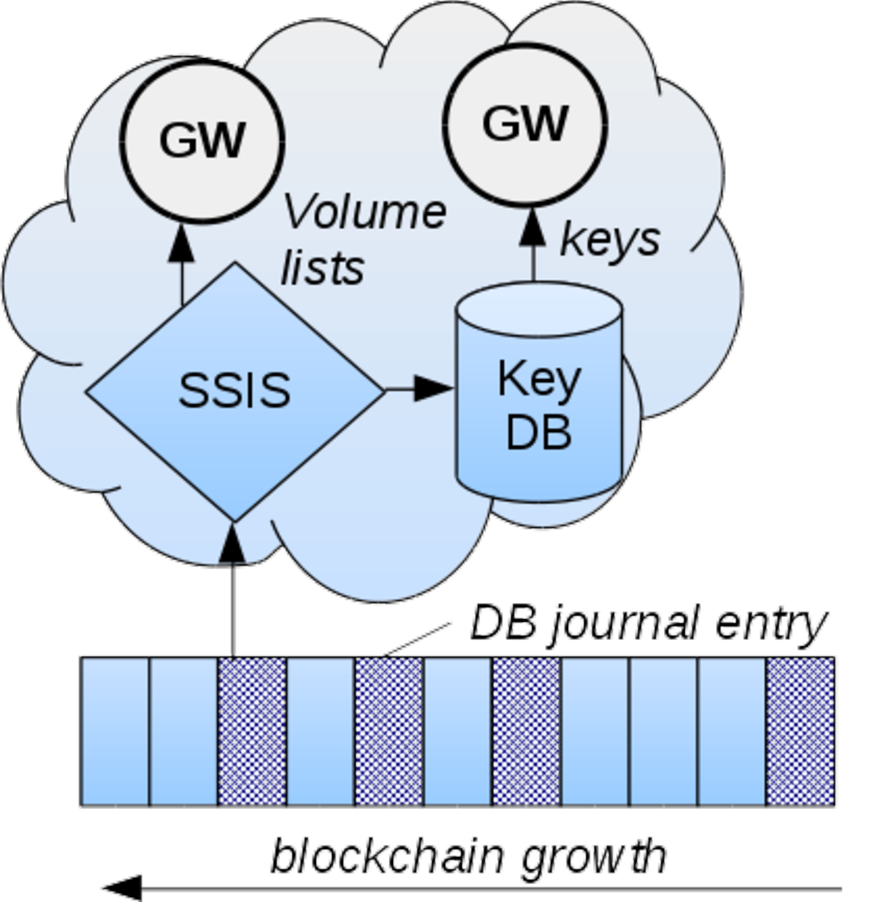
\includegraphics[width=0.47\textwidth]{figures/blockstack-overview}
\caption{\it
   Overview of how a self-sovereign identity system (SSIS) works.  By reading a
   database journal embedded in a proof-of-work blockchain, each SSIS server
   will construct the same database independently.  This gives each
   users the current public keys for all other users.
   }
\label{fig:cert-graph}
\end{figure}

This approach to key distribution ensures that each gateway receives the same
set of user public keys without introducing central points of trust. This is
because practical self-sovereign identity systems rely on proof-of-work
blockchains to construct a tamper-resistant log of key updates for a particular
name.

The security of Waskern is thus underpinned by the practical difficulty of attacking a
PoW blockchain: given two instances of the PoW blockchain,
a peer accepts the one with the most cumulative work (i.e. the
``heaviest'' chain)~\cite{bitcoin-textbook}. As long as no set of peers controls over 50\% of the
compute power used to construct the blockchain, and as long as no blockchain
peers remain partitioned indefinitely, then with extremely high probability two
mutually distrustful peers will independently agree on the heaviest blockchain
simply by inspecting each candidate's proof-of-work.  This in turn means
that two instances of the sovereign identity system that take the same view of
the blockchain will independently construct the same name-to-public-key
mappings, all without requiring users to manage private key revocation
certificates or public key discovery!

A detailed discussion of how a production self-sovereign identity system
works can be found in~\cite{blockstack}.

\subsection{Scaling through Aggregation}

Waskern scales in both the quantity of data and the bandwidth it offers by
aggregating underlying services and individual gateways. RGs scale
horizontally--a single RG can be comprised of many concurrent processes
spread across many hosts, but aggregated behind a single host/port via a
load-balancer. Because UGs translate reads and writes into immutable and
uniquely-named chunks, an RG's total bandwidth can be increased simply by
adding more hosts to run more processes.

AGs scale in a similar manner without needing to directly coordinate. If one AG
process detects and publishes new data, other AG processes learn of it
automatically when the UG requests the new data from them (e.g. the knowledge of
publication is delivered through the UG's request).

A single RG or AG can aggregate other RGs or AGs. Using our social media
example, Alice can enforce maximum retention times by replicating chunks to an
RG that monitors their access frequency, and forwards them along to another RG
that writes them to a cloud storage provider. This separates the orthogonal
tasks of removing unaccessed data and interfacing with cloud storage into two
separate I/O stage implementations, which can be reused independently.

Similarly, Bob can aggregate both of his existing social media accounts by
standing up an AG for each, and then deploying a third AG that combines each
subordinate AG's directory trees into a single directory tree that contains
no duplicate files. In both cases, Alice and Bob both minimize the number of
gateways their UGs need to contact to process I/O flows, and separate orthogonal
storage concerns into reusable components.

\subsection{Fault Tolerance}

Beyond assuming that public-key cryptography is infeasible to crack, we assume
that the self-sovereign identity system is available, and that gateways exhibit
fail-stop behavior when it is not.  Gateways in the same volume already trust one another
with a given set of capabilities, so this fail-stop assumption is
reasonable. The blockchain the default self-sovereign identity system uses (Bitcoin) has over 5,000
known replicas across the world~\cite{coindance} and is the most secure in terms
of money sunk into keeping it safe~\cite{coinmarketcap}, so it is likely to be available.

Under these assumptions, gateways can translate arbitrary service failures
(including misbehavior) into fail-stop conditions, preventing users from
unknowingly relying on an unreliable component.  This is because gateways never
process unauthenticated or stale application data.

The MS holds soft state, so if it goes offline or misbehaves, no data is lost.
Gateways detect equivocation, but allow the
user-supplied I/O logic to determine how to handle it.  If the I/O logic is written such that it does not
need the MS to publish and discover manifests, then gateways can
continue to process I/O flows without it.

Waskern tolerates temporary partitions between the AG and its dataset
if the data has already been proven to exist. UGs periodically ask AGs
to re-validate their views of the dataset.
This way, the AG can deduce whether or not its view is out-of-sync, and
synchronize the view before responding to the UG.

Waskern tolerates failures in individual RGs and back-end storage providers by
having a UG query each RG in the volume when pulling chunks.  If all services
and RGs are offline or misbehaving, then the UG blocks until
at least one comes online again. If all services and RGs permanently fail, then data loss is
unavoidable.

A file's coordinator can crash or become partitioned from other gateways.
The user's I/O logic makes the choice as to whether or not the file becomes unavailable
in this failure mode.  If not, then other coordinator-capable gateways will
automatically race to become the new coordinator if they cannot contact
the current coordinator.  The change-coordinator requests are serialized
through the MS, so at most one change-coordinator request succeeds (and all
losers learn the new coordinator).

There is one pathological case to consider where two sets of gateways are
partitioned, and one gateway in each set believes it is the file's coordinator.
In this scenario, the users are also partitioned from their gateways, and the MS
equivocates between both groups about who is the real coordinator, potentially
enabling both gateways to process conflicting I/O flows.

Irreconcilable write histories can only occur in this scenario if the consistency model
created by the user's data-processing logic is already weak enough to allow 
write-processing when less than a majority of gateways are available.
This means that the consistency model already defines a way to resolve divergent
writes like these, irrespective of it's use in Waskern.

Waskern helps detect potential divergences like this via an asynchronous heartbeat
gossip protocol.  If a gateway does not receive a fresh heartbeat for another gateway after
a timeout, it assumes that it is unavailable and acts accordingly.

The UG offers users a
\texttt{chcoord()} method on its control plane to allow the user or application
to proactively shift coordination responsibility around the volume's
gateways.  A gateway's epoch value is affected by a \texttt{chcoord()}, so other
gateways will process it before handling its next I/O flow.

